% Intended LaTeX compiler: pdflatex
\documentclass[10pt,a4paper,UTF8]{article}
\usepackage{zclorg}
\author{zcl.space}
\date{}
\title{一维随机游动}
\hypersetup{
 pdfauthor={zcl.space},
 pdftitle={一维随机游动},
 pdfkeywords={},
 pdfsubject={},
 pdfcreator={Emacs 25.0.50.1 (Org mode 9.0.5)}, 
 pdflang={English}}
\begin{document}

\maketitle
在\href{definition-of-stochastic-process.org}{随机过程的定义} 一节中,我们定义了基于概率空间\((\Omega,\mathcal{F},P)\)的随机过程\(\{\xi(\omega,t),t\in T\}\)。针对 参数\(T\)和\(\xi_{t}(\omega)\)的状态取值是连续的或者离散的,我们有四种随机过程。

今天,我准备讨论一种随机过程,这种随机过程的参数值是离散的,每个离散时刻的随机变量的可能状态也是离散的。我们称这样的随机过程为离散参数离散值的随机过程。今天的这个过程又叫做一维随机游动。具体描述为:
\begin{problem}
设有一质点在\(x\)轴上做随机游动,即在\(t=0\)时,质点位于\(x\)轴的原点\(0\),在\(t=1,2,\ldots\)时质点可以在\(x\)轴上正向或反向移动一个单位距离。做正向移动一个单位距离的概率为\(p\),做反向移动一个单位距离的概率为\(q = 1-p\)。经过时间\(n\),质点偏离原点的距离为\(k\),为处于\(k\)的概率是多少?
\end{problem}

\begin{answer}
首先,我们画出一个可能的随机游动结果:

\begin{figure}[htbp]
\centering
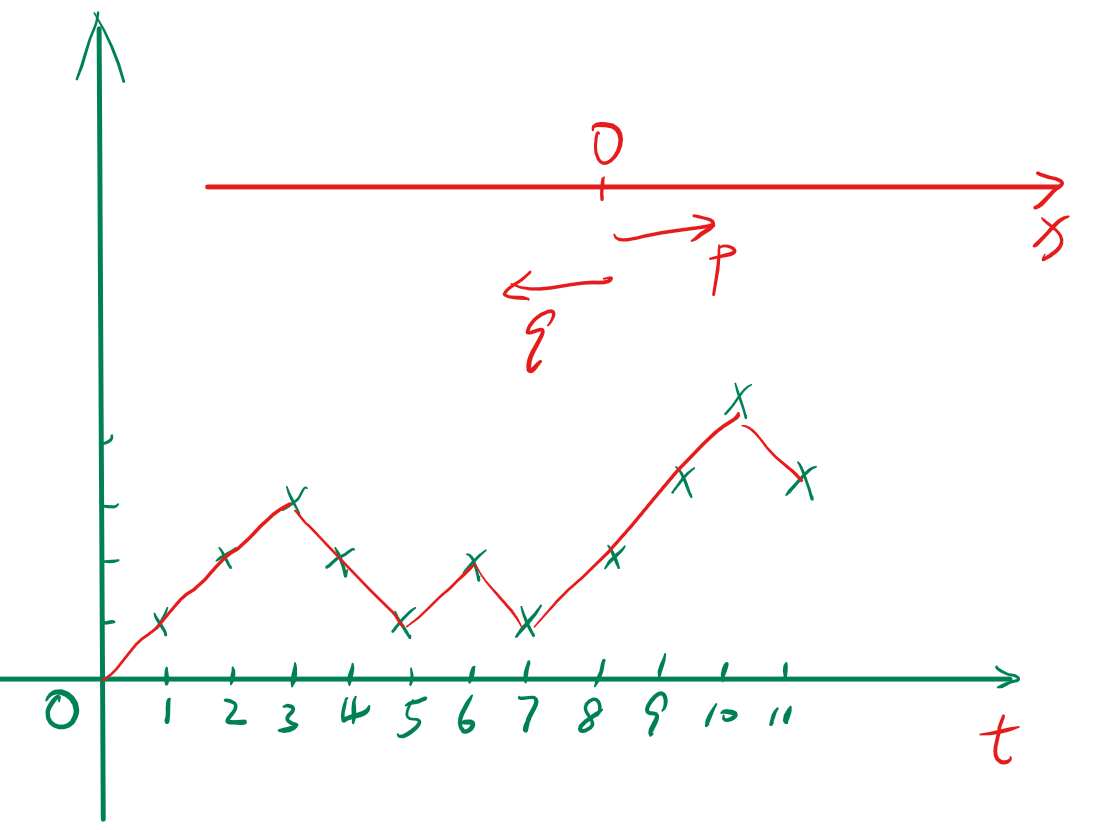
\includegraphics[width=0.6\textwidth]{../../img/math_stochastic/20170418stochastic-one-way-random-walk.png}
\caption{\label{fig:orgf05f2c5}
一个随机游动的样本函数}
\end{figure}

设质点每次移动的距离为\(\xi_{i}\),\(\xi_{i}\)的取值有两种可能\(\{+1,-1\}\),且有:
\begin{eqnarray}
\label{eq:4}
p(\xi_{i} = +1)&=& p \\
p(\xi_{i} = -1)&=& q = 1-p \\
\end{eqnarray}

设质点在\(t=n\)时远离原点的距离是\(\eta_{n}\),则\(\eta_{n}\)也是一个随机变量。于是:
\begin{equation}
\label{eq:1}
\eta_{n} = \sum_{i=1}^{n}\xi_{i},\eta_{0} = 0
\end{equation}

又设质点每次游动与该质点所处的位置无关,当\(i\neq k\)时,\(\xi_{i},\xi_{k}\)是相互统计独立的随机变量。图\ref{fig:orgf05f2c5} 给出了\(\eta_{n}\)的样本函数。

如果在\(n\)次游动中有\(m\)次是正向移动,则\(n-m\)次是反向移动。则:
\begin{equation}
\label{eq:2}
\eta_{n} = \sum_{i=1}^{n}\xi_{i} = m(+1) + (n-m)(-1) = 2m -n = k
\end{equation}

即,\(m = (n+k)/2\)是\(n\)次游动中正向游动的次数。所以有:
\begin{eqnarray}
\label{eq:3}
P(\eta_{n} = k)&=&\binom{n}{m}p^{m}q^{n-m} \\
&=& \binom{n}{\frac{n+k}{2}}p^{\frac{n+k}{2}}q^{\frac{n-k}{2}}
\end{eqnarray}

上式中\(m\)是正整数,说明\(n,k\)同奇偶。
\end{answer}
\end{document}
